\documentclass[11pt,a4paper]{article}
\usepackage[margin=2.5cm]{geometry}
\usepackage{graphicx}
\usepackage{amsmath,amssymb}
\usepackage{booktabs}
\usepackage{hyperref}
\usepackage{float}

\title{A* Island Simulator: Empirical Analysis of Game Mechanics}
\author{Data Analysis Report}
\date{March 2026}

\begin{document}
\maketitle

\begin{abstract}
We analyze 45 replay datasets (9 rounds $\times$ 5 seeds, 51 frames each) to reverse-engineer the simulation mechanics of A* Island. We isolate the effects of food production, winter, settlement spawning, and raiding by examining step-to-step transitions. All findings are supported by reproducible scripts in \texttt{data-analysis/}.
\end{abstract}

%% ============================================================
\section{Food Production and Winter}
\label{sec:food}
\textit{Script: \texttt{analyze\_food\_deep.py}}

\subsection{Food Production Formula}
We filter to non-raided, alive, same-owner transitions ($N = 190{,}079$) and compare several linear models for $\Delta f = f_{t+1} - f_t$. The key finding is that \textbf{terrain effects scale with $(1-f)$}, i.e.\ food production is dampened when food is already high. This improved $R^2$ from 0.51 to 0.71.

Best linear model (Model D, $R^2 = 0.714$):
\begin{equation}
\Delta f = \underbrace{0.031}_{\text{base}} \underbrace{- 0.131 \cdot p}_{\text{pop cost}} + \underbrace{0.683 \cdot f(1{-}f)}_{\text{feedback}} + \underbrace{(0.050 \cdot n_P + 0.088 \cdot n_F - 0.004 \cdot n_M - 0.020 \cdot n_S)(1{-}f)}_{\text{terrain}} + w_{r,s,t}
\end{equation}
where $p$ = population, $f$ = food, $n_P, n_F, n_M, n_S$ = adjacent plains, forest, mountain, and settlement counts, and $w_{r,s,t}$ is a stochastic weather component constant within each (round, seed, step) group.

\begin{table}[H]
\centering
\caption{Food model coefficient stability across 9 rounds.}
\begin{tabular}{lrrr}
\toprule
Coefficient & Mean & Std & CV \\
\midrule
\texttt{pop} & $-0.145$ & 0.022 & 0.15 \\
\texttt{food$\times$(1-food)} & $+0.781$ & 0.157 & 0.20 \\
\texttt{plains$\times$(1-f)} & $+0.050$ & 0.004 & 0.07 \\
\texttt{forest$\times$(1-f)} & $+0.088$ & 0.006 & 0.07 \\
\texttt{mountain$\times$(1-f)} & $-0.003$ & 0.004 & 1.30 \\
\texttt{settl$\times$(1-f)} & $-0.012$ & 0.009 & 0.76 \\
\texttt{is\_port} & $+0.009$ & 0.006 & 0.73 \\
\bottomrule
\end{tabular}
\label{tab:food_coefs}
\end{table}

The terrain coefficients (plains, forest) are highly stable across rounds (CV $\leq 7\%$). The feedback term and intercept vary more, likely because they absorb round-specific parameter differences.

\subsection{Weather and Winter}
Using fixed-effects estimation (demeaning by round/seed/step), we extract the weather component $w_{r,s,t}$:
\begin{itemize}
\item Mean: $+0.007$, Std: $0.045$, Range: $[-0.14, +0.13]$
\item Within-group residual std: $0.068$ (remaining settlement-level noise)
\item Weather is approximately i.i.d.\ normal across steps, with no trend over time
\end{itemize}

The intercept of $+0.031$ represents $\text{food\_base} - \text{winter\_severity}$. From newborn ruin settlements (unraided, $N = 10{,}075$), which start with food $\approx 0$ and receive one round of food production plus winter, we estimate child food $= 0.136 \pm 0.052$. This is consistent with $\text{winter} \approx 0.01$--$0.02$ per step---a small effect relative to food production.

\begin{figure}[H]
\centering
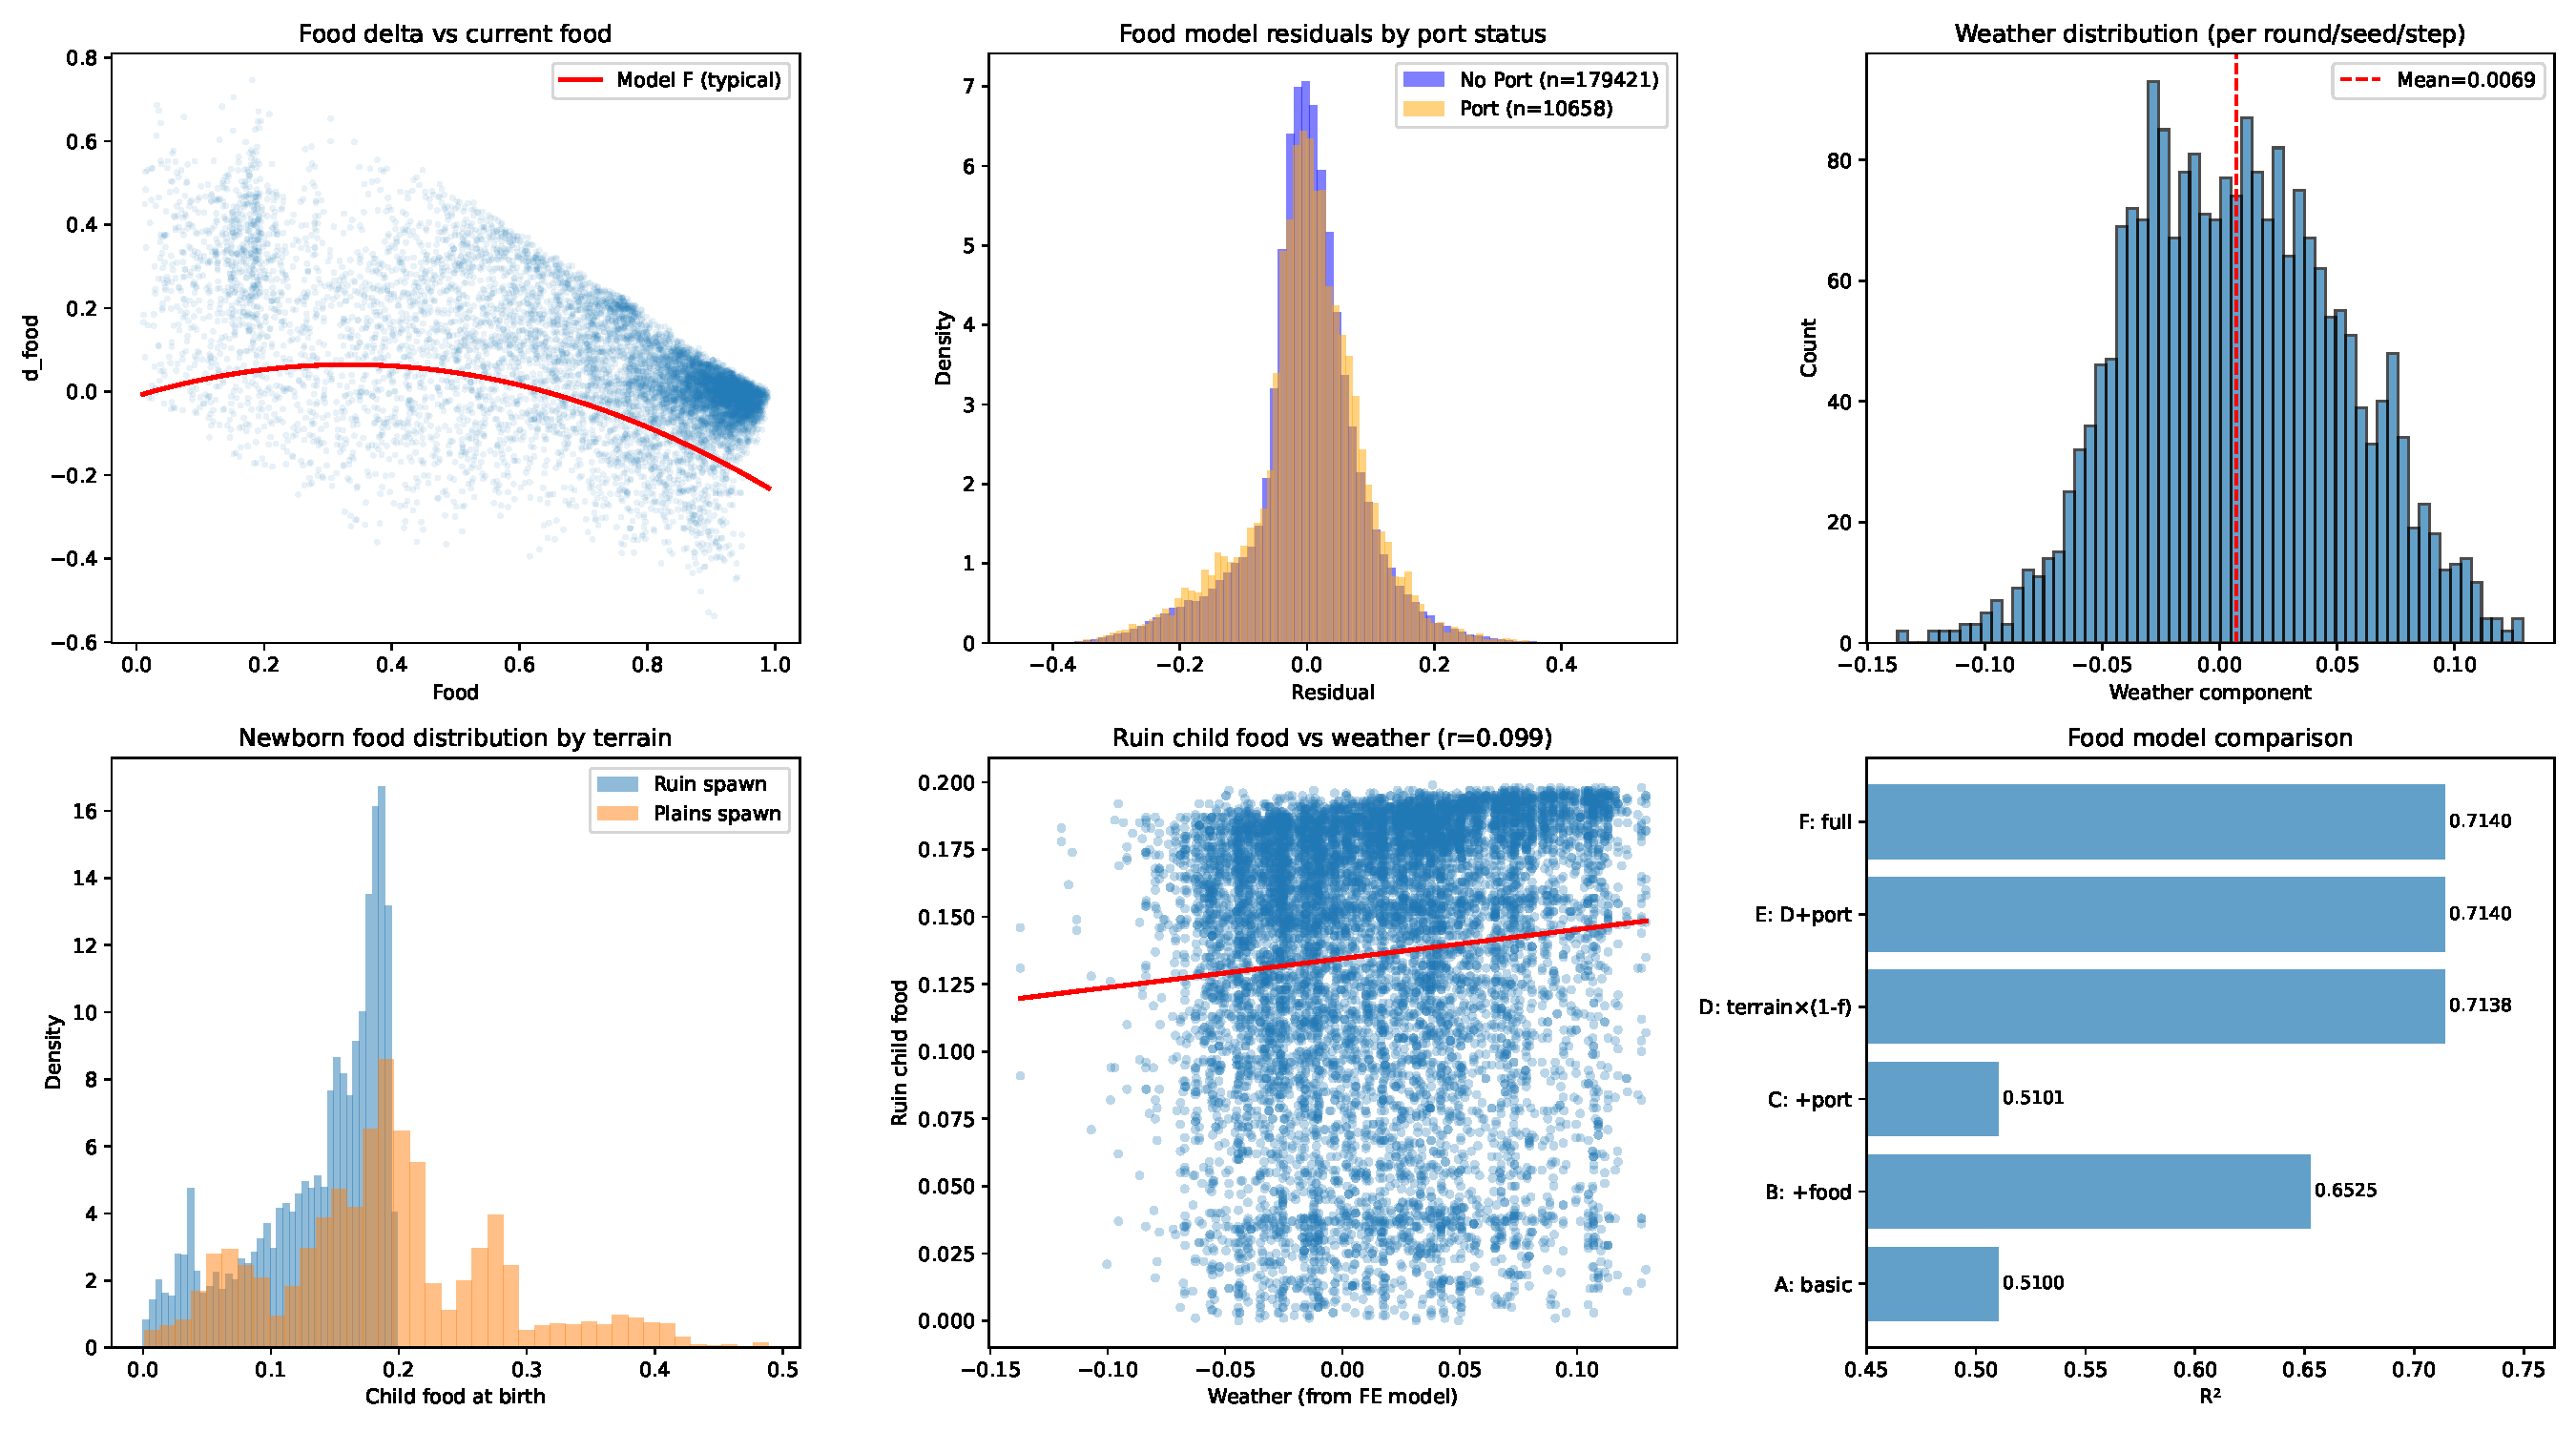
\includegraphics[width=\textwidth]{plots/food_deep_analysis.pdf}
\caption{Food model analysis. Top-left: $\Delta f$ vs $f$ with model overlay. Top-middle: residuals by port status. Top-right: weather distribution. Bottom-left: newborn food by terrain. Bottom-middle: ruin child food vs weather ($r = 0.10$). Bottom-right: model comparison.}
\label{fig:food}
\end{figure}

%% ============================================================
\section{Settlement Spawning}
\label{sec:spawn}
\textit{Scripts: \texttt{analyze\_spawn.py}, \texttt{analyze\_spawn\_pspawn.py}}

\subsection{Spawn Probability}
From 227,719 alive settlement-steps, 22,021 resulted in a spawn (9.67\%). The spawn probability is well approximated by:
\begin{equation}
P(\text{spawn}) \approx 0.124 \cdot p \cdot f
\end{equation}
This is roughly linear in both population and food, though it saturates at high population ($p > 4$) and drops at very high food ($f > 0.85$). Available buildable terrain nearby (plains + forest + ruin) is a prerequisite: $P(\text{spawn})$ drops to near zero with no buildable neighbors. Defense, wealth, and port status have no direct effect.

\begin{figure}[H]
\centering
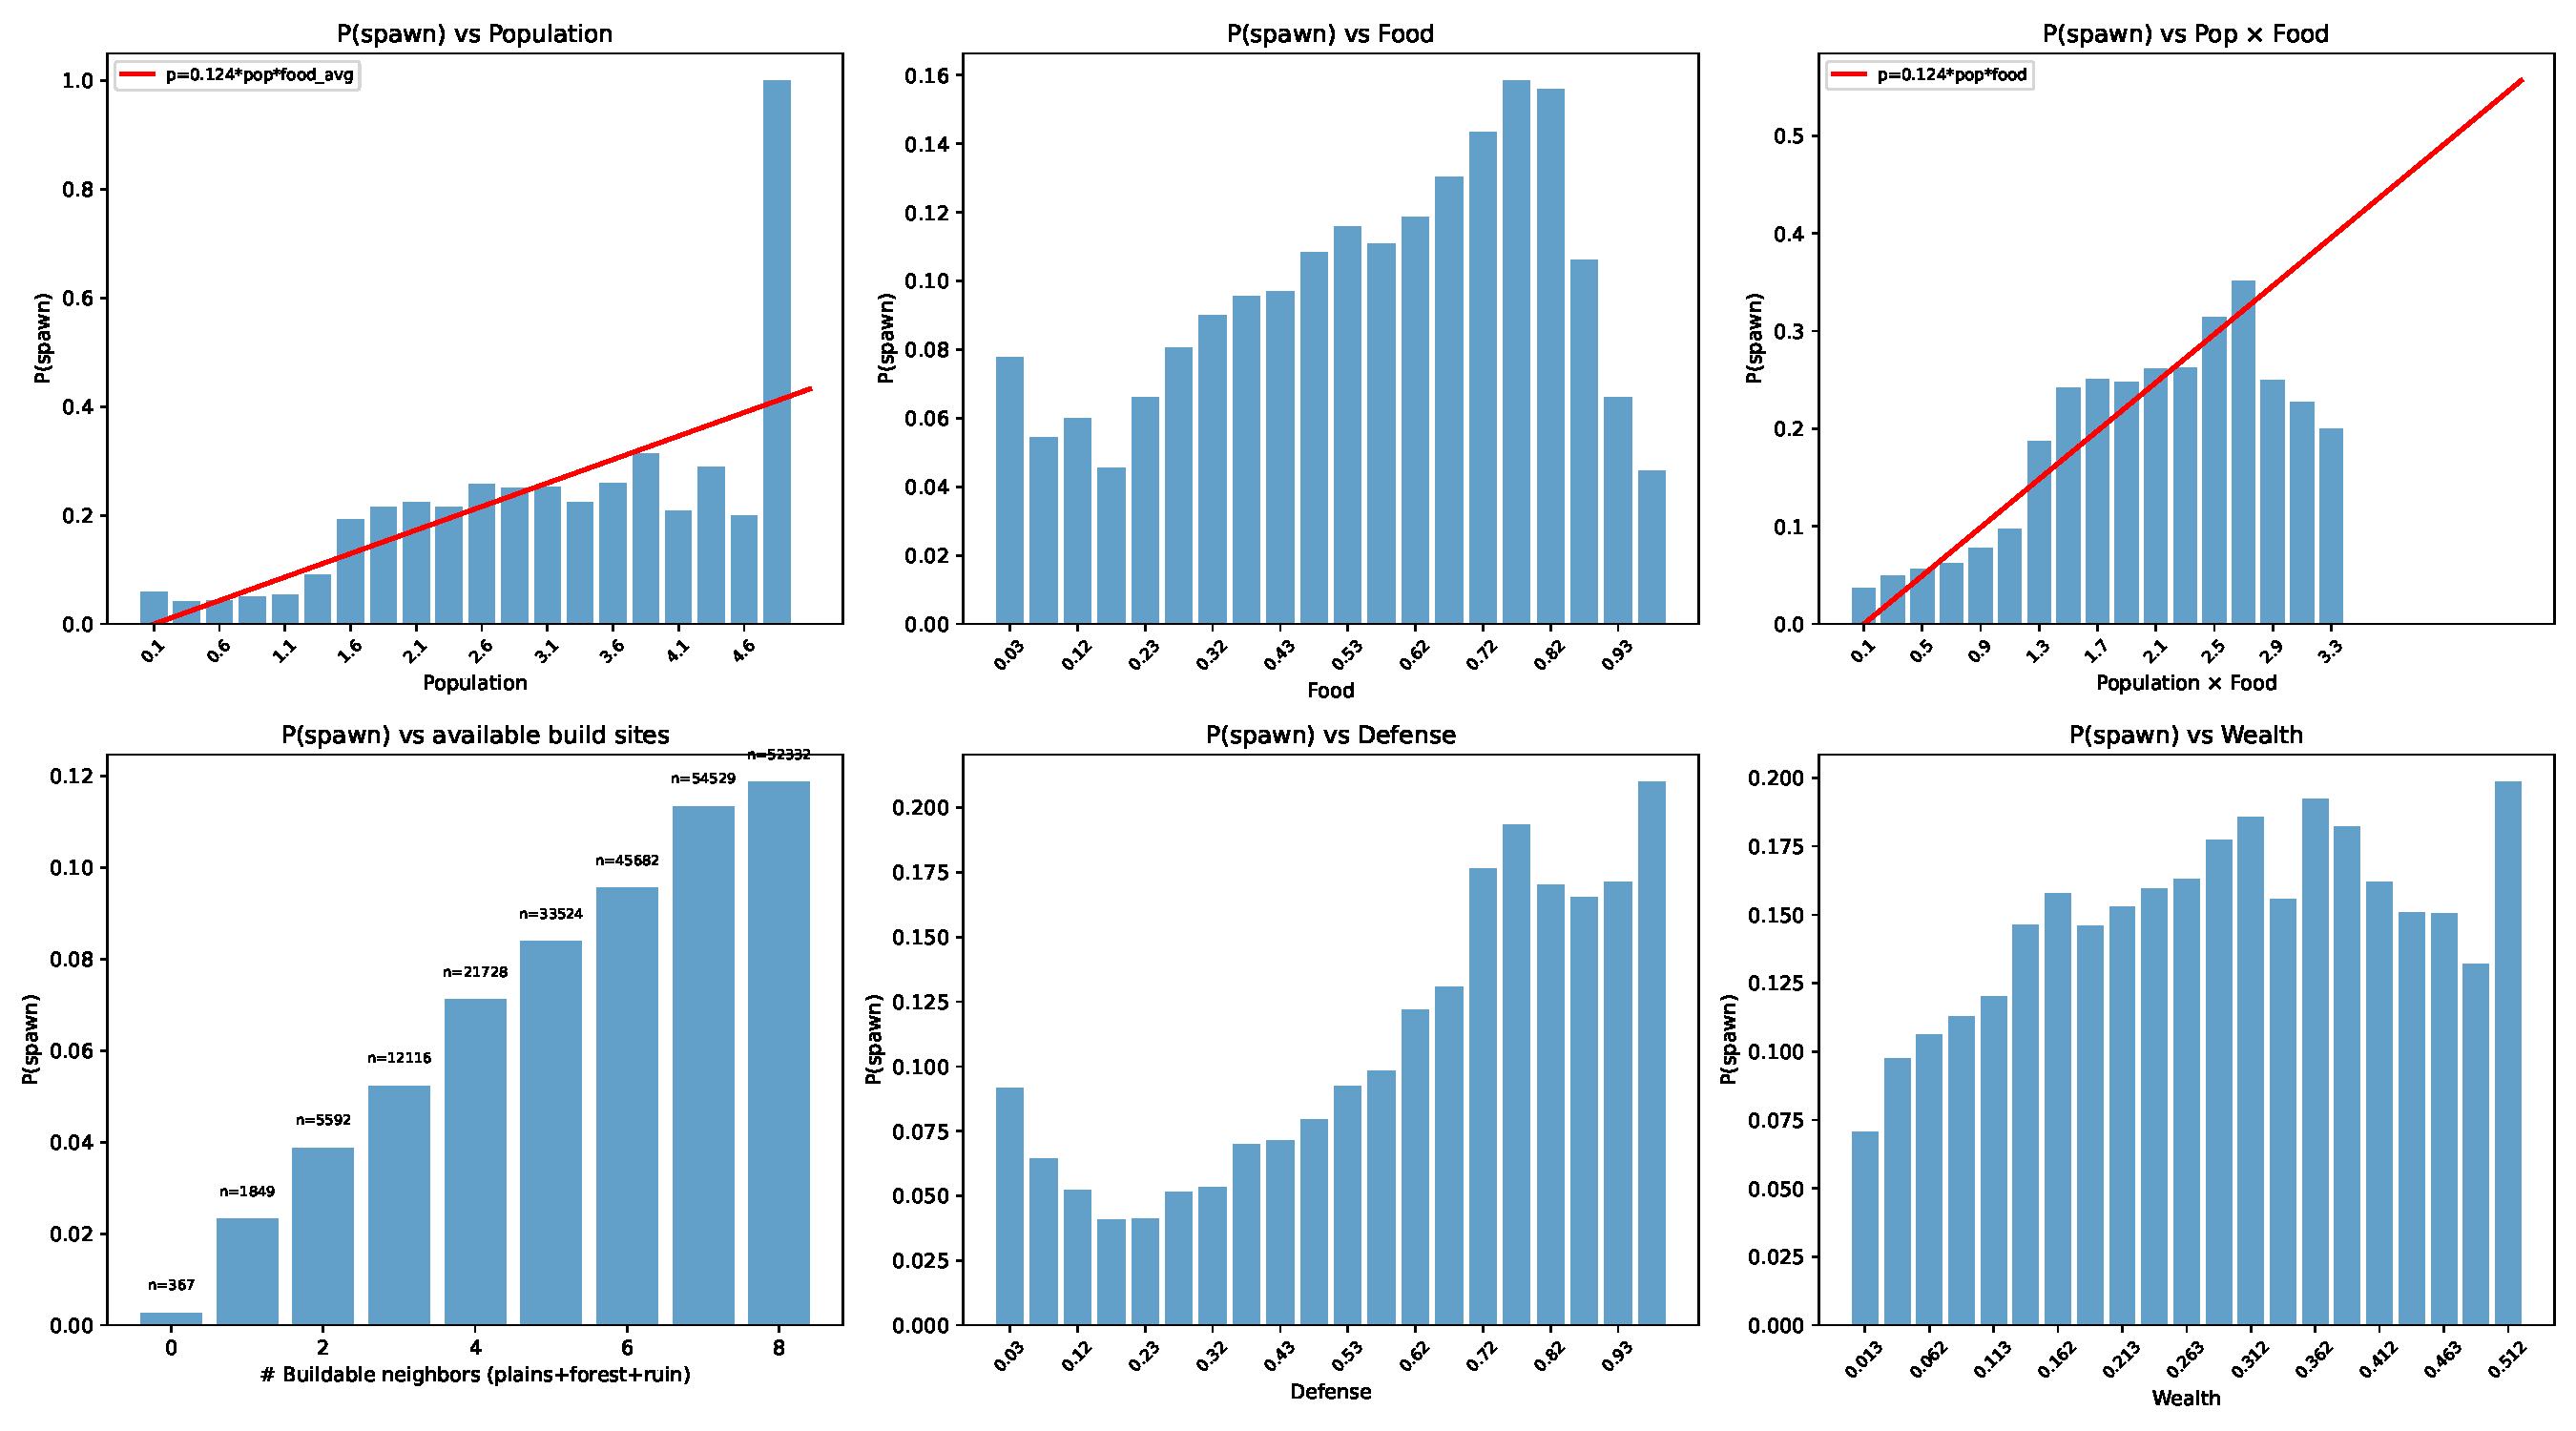
\includegraphics[width=\textwidth]{plots/spawn_pspawn.pdf}
\caption{Spawn probability as a function of population, food, their product, buildable neighbors, defense, and wealth.}
\label{fig:pspawn}
\end{figure}

\subsection{Parent and Child Effects}
\textbf{Parent cost.} Spawning parents lose $\sim 0.05$ extra population compared to non-spawning settlements ($\Delta p_{\text{spawn}} = -0.063$ vs $\Delta p_{\text{no-spawn}} = -0.011$). Food and wealth are not directly affected.

\textbf{Child stats.} Child stats are deterministic by the terrain the child spawns on:

\begin{table}[H]
\centering
\caption{Child settlement initial stats by terrain type.}
\begin{tabular}{lrrrr}
\toprule
Terrain & Population & Defense & Food & Wealth \\
\midrule
Ruin ($N = 10{,}075$) & 0.400 (exact) & 0.150 (exact) & $0.136 \pm 0.052$ & $0.007 \pm 0.011$ \\
Plains ($N = 10{,}164$) & $0.488 \pm 0.033$ & $0.193 \pm 0.017$ & $0.181 \pm 0.088$ & $0.031 \pm 0.034$ \\
Forest ($N = 3{,}846$) & $0.488 \pm 0.033$ & $0.193 \pm 0.017$ & $0.183 \pm 0.086$ & $0.031 \pm 0.034$ \\
\bottomrule
\end{tabular}
\label{tab:child_stats}
\end{table}

Ruin children have \emph{exactly} pop $= 0.4$, def $= 0.15$. Plains/forest children have pop $\approx 0.5$, def $\approx 0.2$, with small variation from post-spawn raids and winter. Child food is weakly correlated with parent food ($r = 0.28$) and terrain neighbors.

\subsection{Spawn Terrain and Distance}
New settlements spawn on: Plains (42.2\%), Ruin (41.8\%), Forest (16.0\%). Approximately 1\% of coastal spawns become ports. The parent-child Chebyshev distance is: 1 (65\%), 2 (26\%), 3+ (9\%).

\begin{figure}[H]
\centering
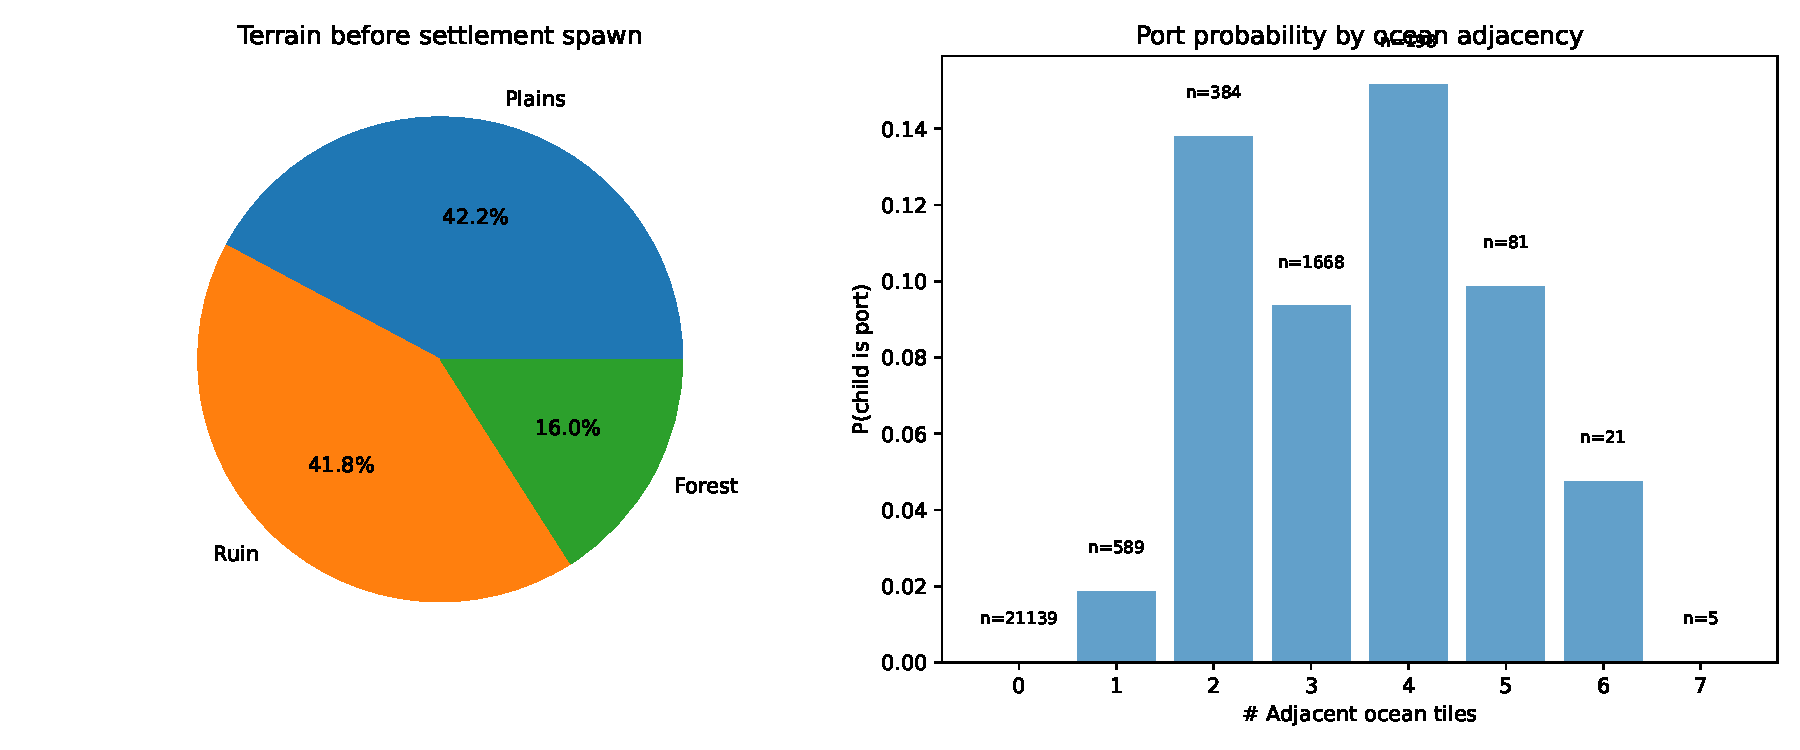
\includegraphics[width=\textwidth]{plots/spawn_terrain.pdf}
\caption{Left: terrain distribution before spawn. Right: port probability by ocean adjacency.}
\label{fig:terrain}
\end{figure}

%% ============================================================
\section{Raid Mechanics}
\label{sec:raids}
\textit{Script: \texttt{analyze\_raids\_v2.py}}

We detect raids as transitions with $\Delta \text{defense} < -0.01$, identifying 18,485 raid events (8.8\% of alive settlements per step).

\subsection{Defense Recovery}
Non-raided settlements show defense \emph{growth} approximately proportional to current defense:

\begin{table}[H]
\centering
\caption{Defense recovery by defense level (non-raided settlements).}
\begin{tabular}{ccc}
\toprule
Defense bin & Mean $\Delta$defense & $N$ \\
\midrule
0.1--0.2 & $+0.016$ & 11{,}496 \\
0.2--0.3 & $+0.023$ & 21{,}298 \\
0.4--0.5 & $+0.044$ & 7{,}922 \\
0.6--0.7 & $+0.059$ & 5{,}208 \\
0.8--0.9 & $+0.069$ & 3{,}300 \\
0.95--1.0 & $+0.002$ & 40{,}541 \\
\bottomrule
\end{tabular}
\label{tab:def_recovery}
\end{table}

Defense grows roughly as $\Delta d \approx 0.08 \cdot d$, capped at $d = 1.0$. A quadratic model $\Delta d = 0.349 d - 0.276 d^2$ achieves $R^2 = 0.59$ (non-raided, $N = 190{,}161$).

\subsection{Raid Damage}

\textbf{Defender effects (unsuccessful raids, $N = 17{,}477$):}
\begin{itemize}
\item Defense: $\Delta d = -0.024$ (single raid), $\Delta d = -0.094$ (2+ raids)
\item Population: survival ratio $\text{pop}_{t+1}/\text{pop}_t \approx 0.91$ (single), $\approx 0.86$ (heavy)
\item Wealth: $\Delta w \approx -0.34 \times w$ (proportional to defender wealth)
\item Food: \textbf{not directly affected} by raids ($\Delta f_{\text{raided}} \approx \Delta f_{\text{non-raided}}$)
\end{itemize}

\textbf{Defender effects (successful raids / takeover, $N = 1{,}008$):}
\begin{itemize}
\item Mean $\Delta d = -0.059$, mean $\Delta p = -0.088$, mean $\Delta w = -0.029$
\item Takeover probability decreases with post-raid defense but can occur up to $d_{\text{after}} \approx 0.42$ (95th percentile)
\end{itemize}

\textbf{Attacker effects} cannot be cleanly isolated because the nearest enemy may not be the actual attacker, and attacker changes include natural food/pop growth. From the raw data, attackers gain small amounts of wealth ($+0.004$ mean).

\begin{figure}[H]
\centering
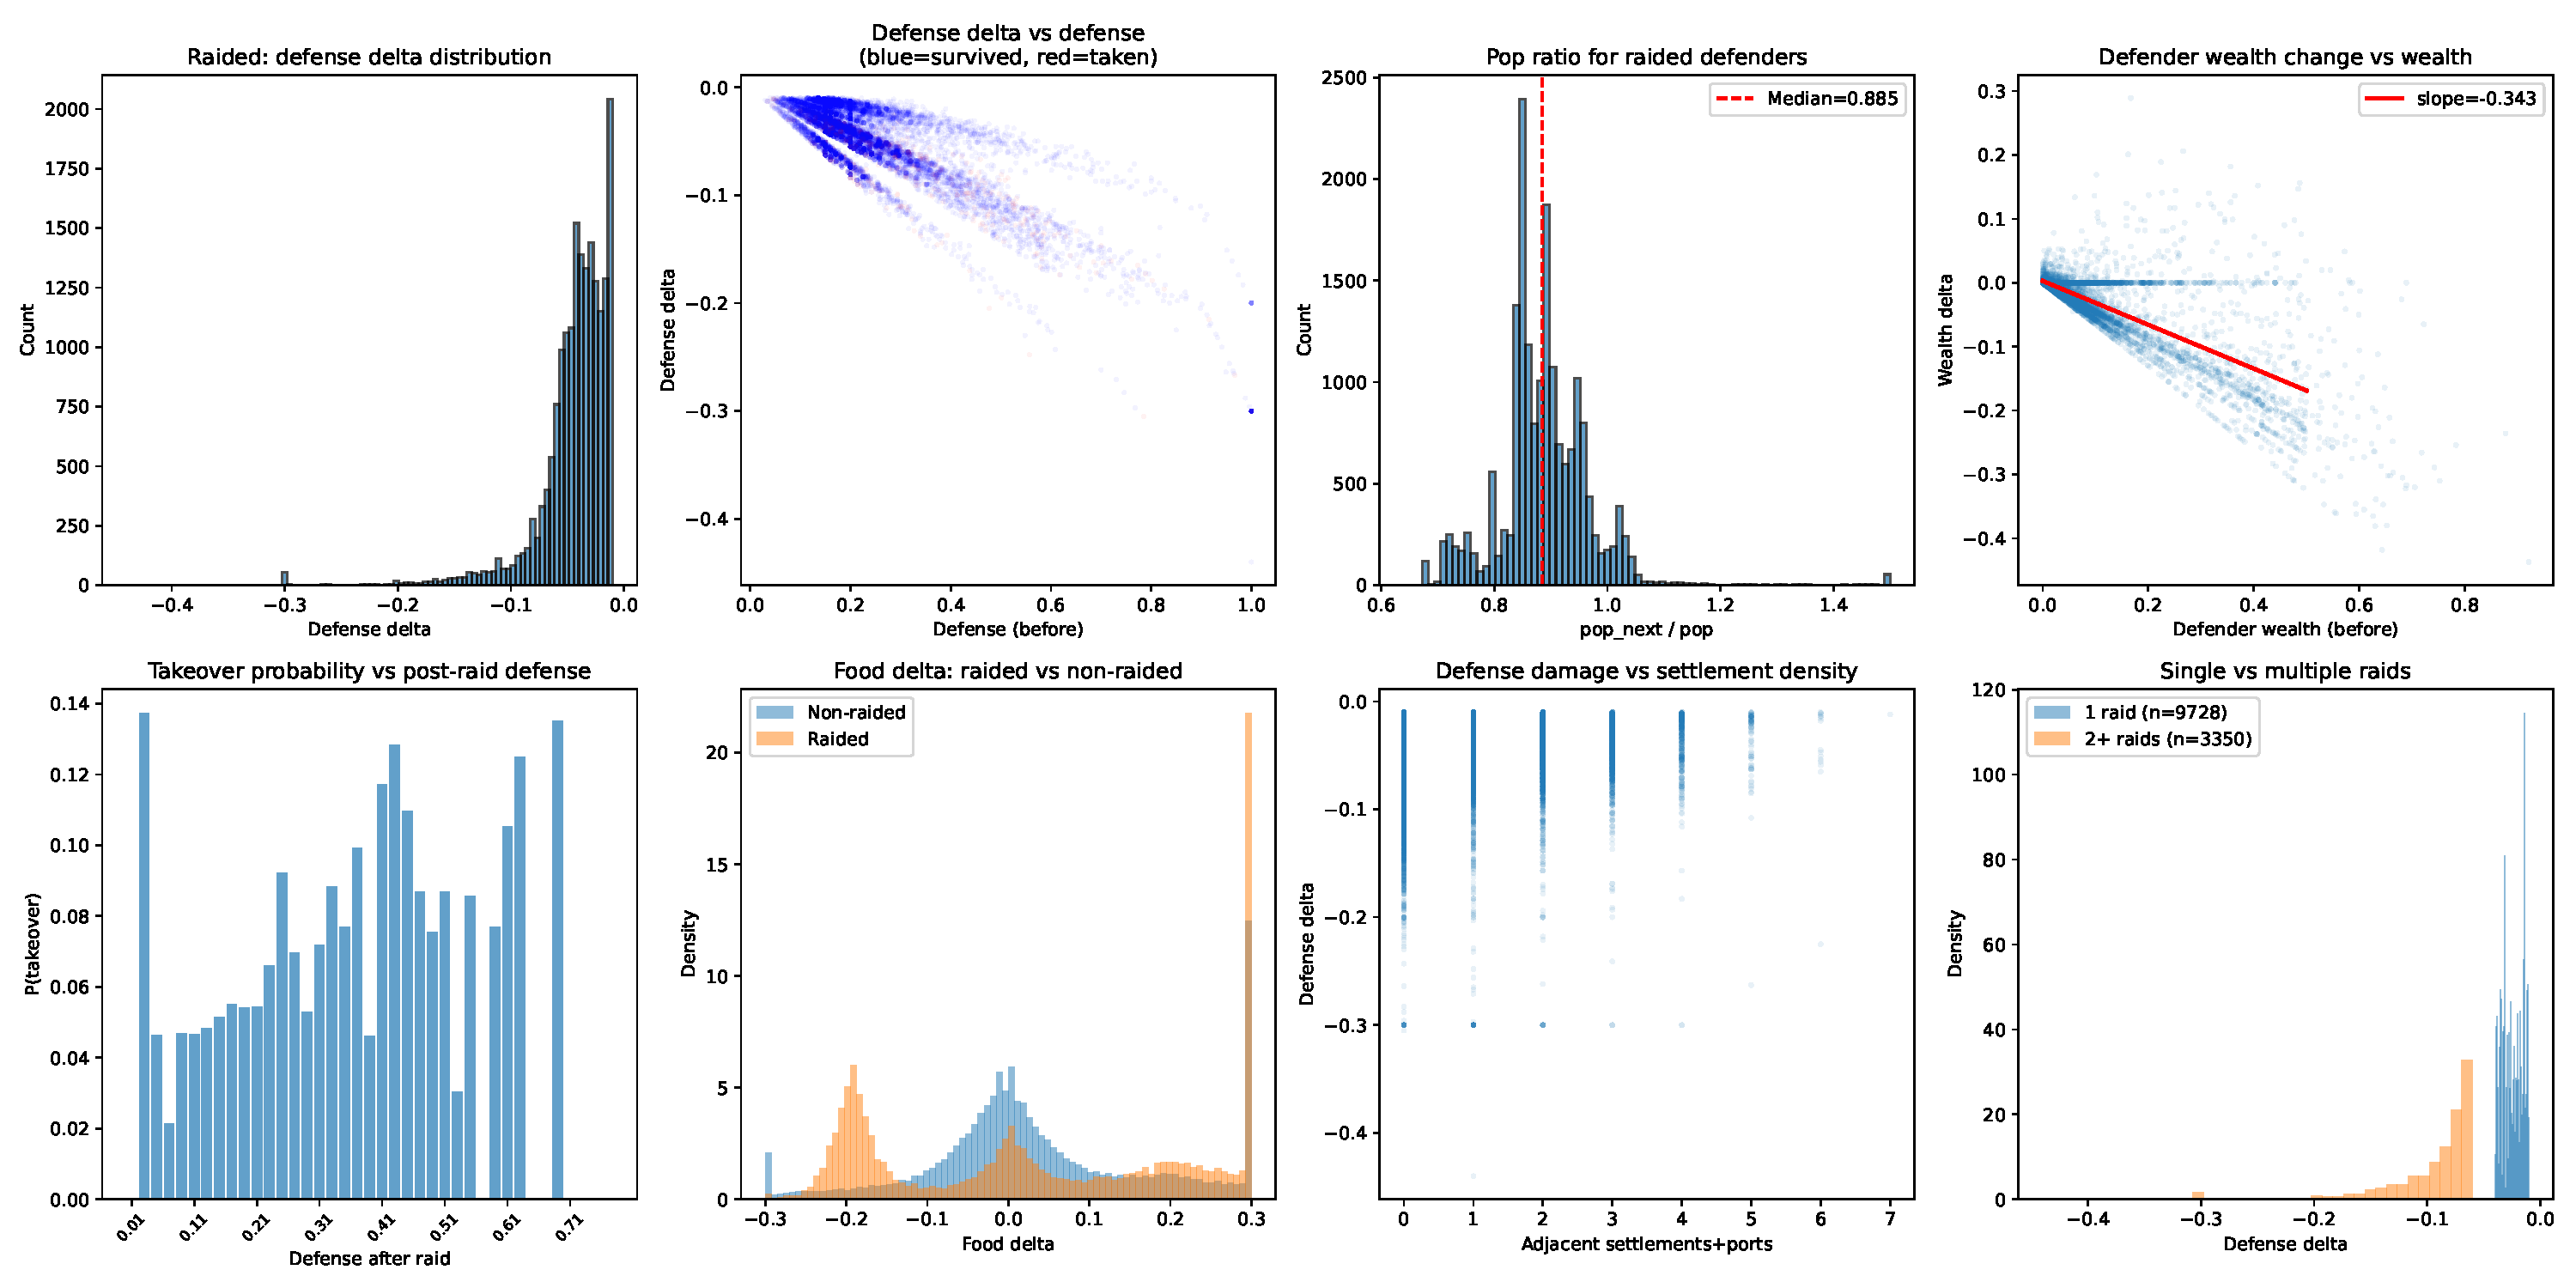
\includegraphics[width=\textwidth]{plots/raid_analysis_v2.pdf}
\caption{Raid mechanics. Top row: defense delta distribution, defense delta vs defense (blue = survived, red = taken), pop survival ratio, wealth change. Bottom row: takeover probability, food delta comparison, damage vs density, single vs multiple raids.}
\label{fig:raids}
\end{figure}

%% ============================================================
\section{Model Quality Comparison}
\label{sec:worst}
\textit{Script: \texttt{analyze\_worst\_modeled.py}}

\begin{table}[H]
\centering
\caption{Best linear model $R^2$ for each variable (non-raided, $N = 190{,}161$).}
\begin{tabular}{lrrrr}
\toprule
Variable & $R^2$ (Linear) & MAE & RMSE & $R^2$ (GBM CV) \\
\midrule
Food & \textbf{0.714} & 0.061 & 0.086 & 0.740 \\
Defense & 0.593 & 0.012 & 0.016 & 0.206 \\
Wealth & 0.021 & 0.005 & 0.015 & 0.074 \\
Population & \textit{0.011} & 0.051 & 0.084 & 0.028 \\
\bottomrule
\end{tabular}
\label{tab:model_comparison}
\end{table}

\textbf{Population is the worst-modeled variable} ($R^2 = 0.01$). Even gradient boosting achieves only $R^2 = 0.03$. The reason: population changes are dominated by stochastic events (spawning costs, raids) that are binary and unpredictable from the current state alone. The deterministic growth component ($\Delta p \approx 0.02 \cdot f \cdot (1 - p/5)$) is small relative to these shocks.

\textbf{Wealth} is similarly hard to predict ($R^2 = 0.02$), driven by stochastic trade and raid events.

\textbf{Defense} has a strong quadratic model ($R^2 = 0.59$) but GBM overfits (train $R^2 = 0.83$ vs CV $R^2 = 0.21$), indicating that non-raided defense dynamics are well captured by $\Delta d \approx 0.35 d - 0.28 d^2$ but additional features add noise, not signal.

\textbf{Food} is the best modeled ($R^2 = 0.71$), with terrain$\times(1{-}f)$ being the key insight. GBM only marginally improves it ($R^2 = 0.74$), suggesting the linear model captures most of the structure.

\begin{figure}[H]
\centering
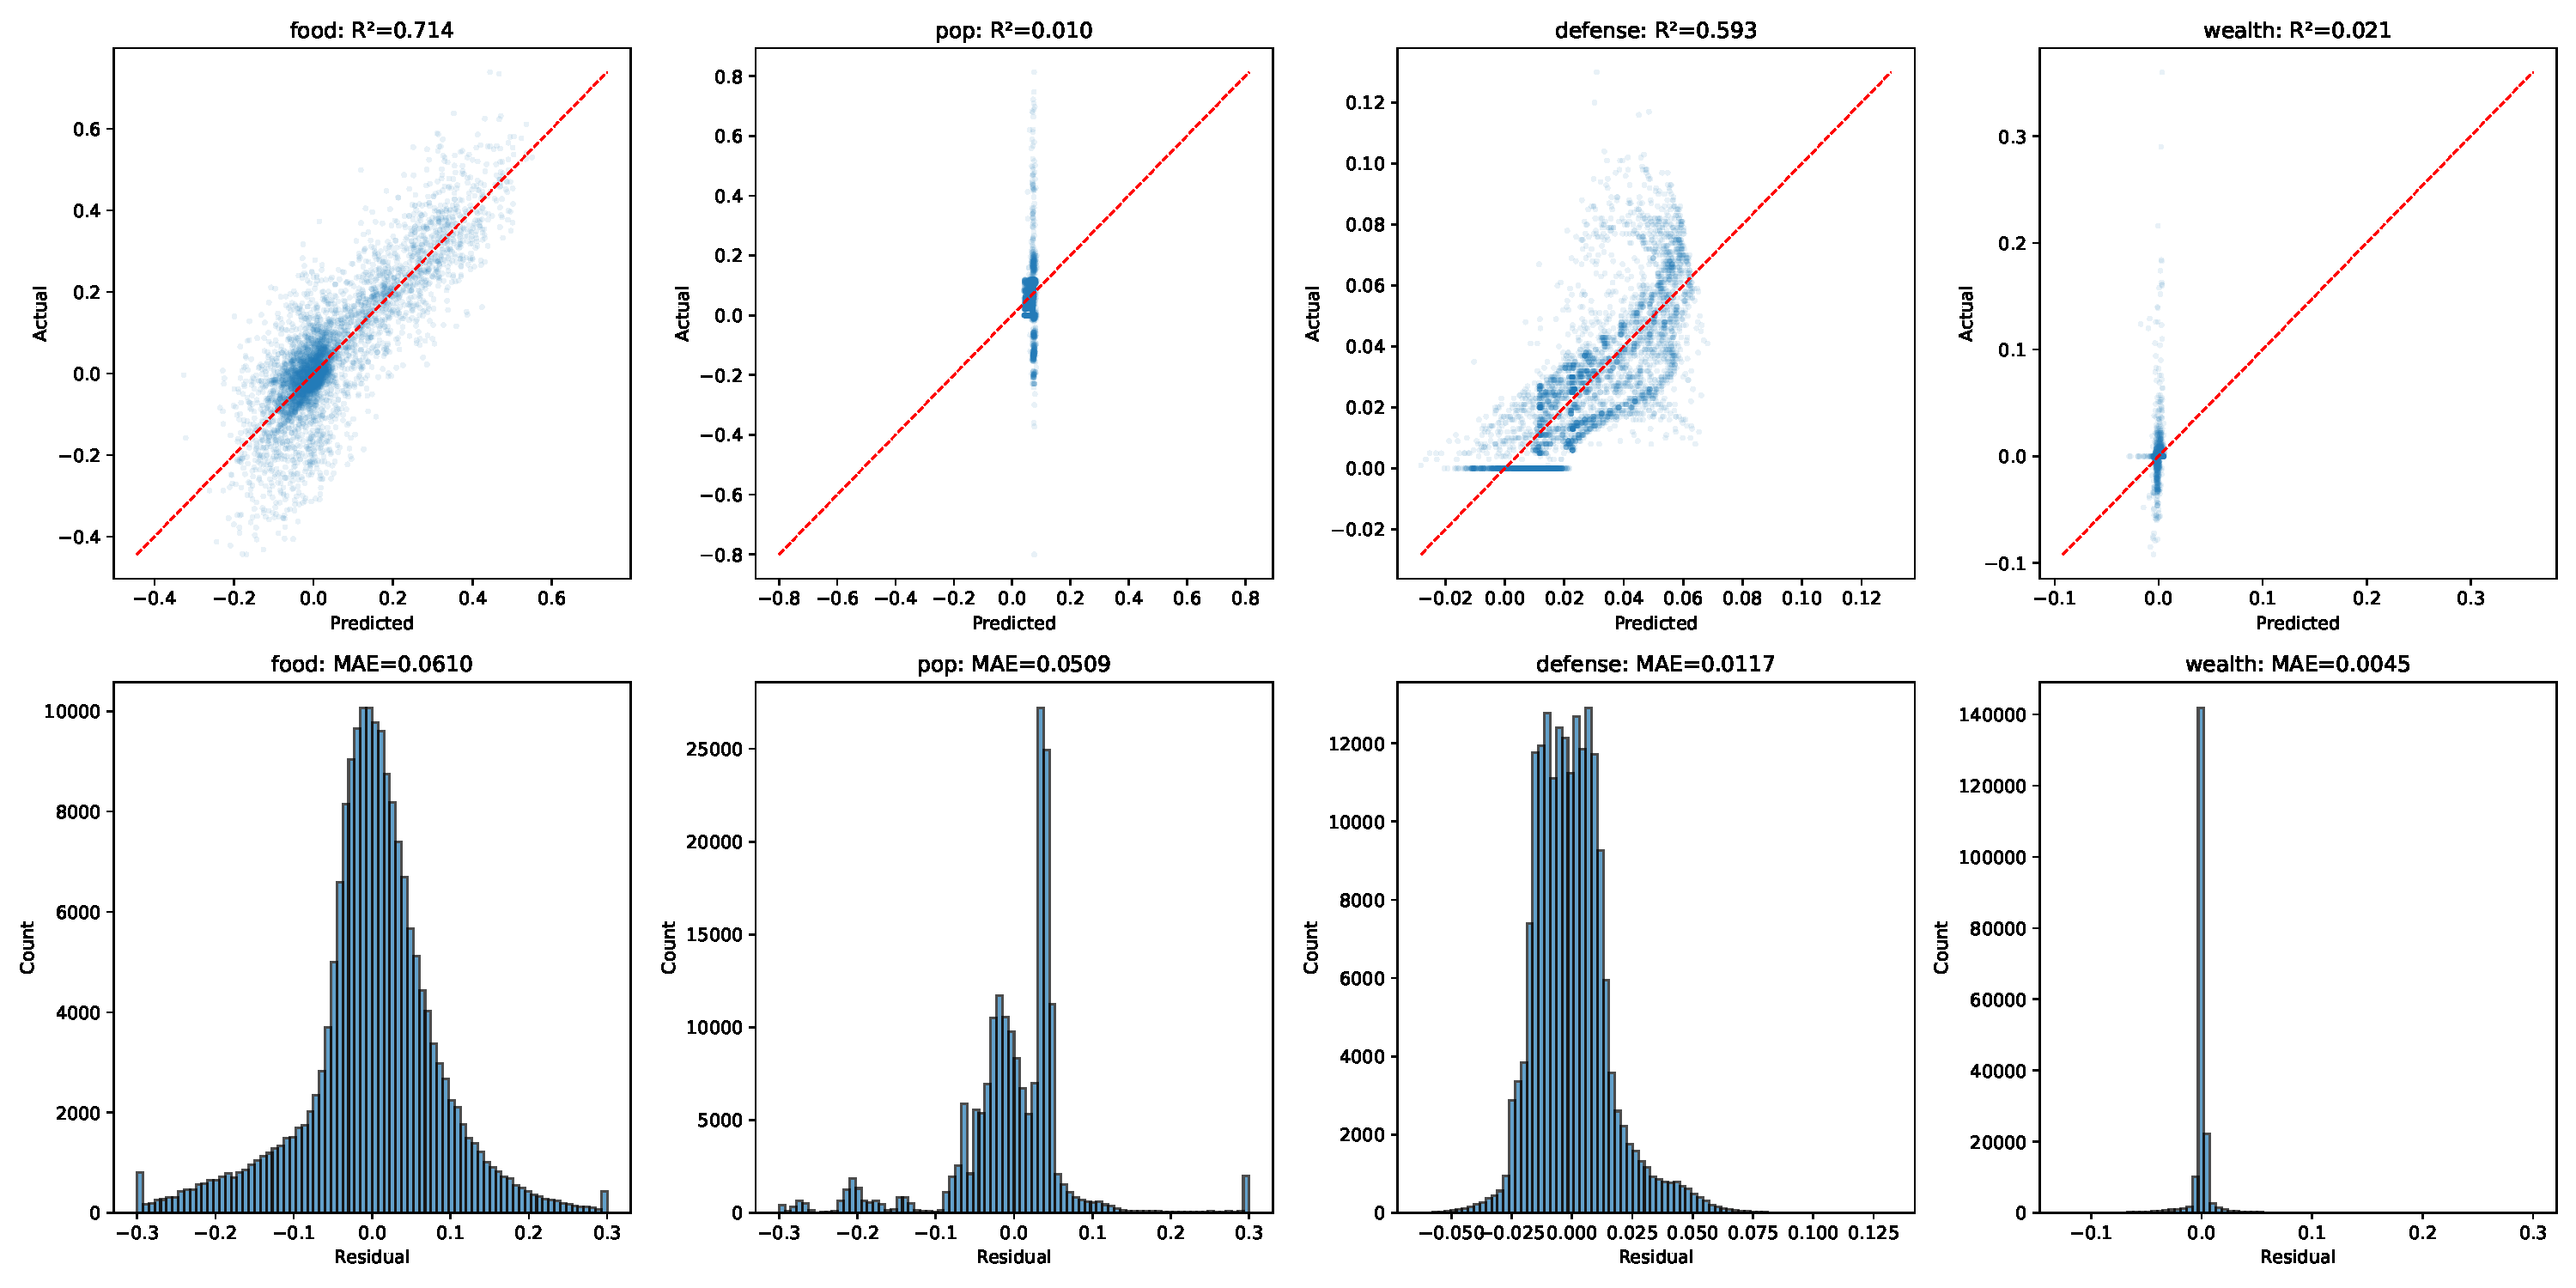
\includegraphics[width=\textwidth]{plots/worst_modeled.pdf}
\caption{Model quality for all four variables. Top: predicted vs actual. Bottom: residual distributions.}
\label{fig:worst}
\end{figure}

The large population residuals occur disproportionately at high pop ($\bar{p} = 1.94$ vs 1.15 normal) and high defense ($\bar{d} = 0.82$ vs 0.49), consistent with spawning parents who stochastically lose population.

%% ============================================================
\section{Summary of Key Parameters}
\label{sec:params}

\begin{table}[H]
\centering
\caption{Estimated game parameters from data.}
\begin{tabular}{llr}
\toprule
Parameter & Description & Estimated Value \\
\midrule
\texttt{food\_base} - \texttt{winter} & Net food intercept & $+0.031$ \\
\texttt{food\_pop\_coeff} & Population food cost & $-0.131$ \\
\texttt{food\_feedback} & Food autoregulation $f(1{-}f)$ & $+0.683$ \\
\texttt{food\_plains} $\times (1{-}f)$ & Plains adjacency effect & $+0.050$ \\
\texttt{food\_forest} $\times (1{-}f)$ & Forest adjacency effect & $+0.088$ \\
\texttt{weather\_std} & Per-step food noise & $0.045$ \\
\texttt{growth\_prob} & Spawn coefficient & $0.124 \times p \times f$ \\
\texttt{parent\_cost} & Pop cost of spawning & $\sim 0.05$ \\
\texttt{ruin\_child\_pop} & Ruin child population & $0.400$ \\
\texttt{ruin\_child\_def} & Ruin child defense & $0.150$ \\
\texttt{plains\_child\_pop} & Plains/forest child population & $0.500$ \\
\texttt{plains\_child\_def} & Plains/forest child defense & $0.200$ \\
\texttt{defense\_growth} & Defense growth rate & $\sim 0.08 \cdot d$ \\
\texttt{raid\_pop\_survival} & Pop retention per raid & $\sim 0.91$ \\
\texttt{raid\_wealth\_fraction} & Wealth stolen per raid & $\sim 0.34 \times w$ \\
\bottomrule
\end{tabular}
\label{tab:params}
\end{table}

\section*{Reproducibility}
All analysis scripts are in \texttt{data-analysis/}:
\begin{itemize}
\item \texttt{load\_replays.py} --- shared data loader (transition, spawn, raid DataFrames)
\item \texttt{analyze\_food\_deep.py} --- food model comparison, weather extraction, winter severity
\item \texttt{analyze\_spawn.py} --- spawn statistics, parent/child effects, terrain distribution
\item \texttt{analyze\_spawn\_pspawn.py} --- spawn probability functional form, child food determinants
\item \texttt{analyze\_raids\_v2.py} --- raid detection, defense damage, pop survival, wealth, takeover
\item \texttt{analyze\_worst\_modeled.py} --- cross-variable model comparison, GBM benchmark
\end{itemize}

\end{document}
